The goal of each experiment was, to trace the current consumption of the ESP8266 during different tasks.
For this, we used the following experimental setup:

\begin{figure}[h]
    \centering
    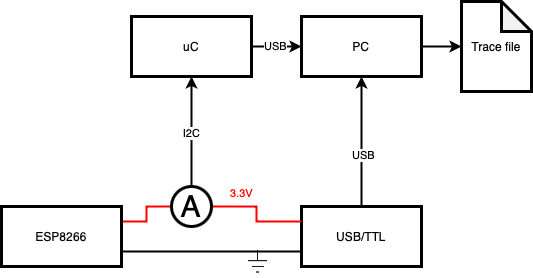
\includegraphics[width = \linewidth]{fig/experimental_setup.png}
    \caption{Setup to measure the current consumption of the ESP8266.}
    \label{fig:experiment_setup}
\end{figure}

The Amperemeter consisted of an INA219 module together with a shunt resistor of $R_{shunt} = 2.2 \Omega$.
With a maximum current consumtion of $I_{max}=170 mA$ \cite{espressif_inc_esp8266_2016}, the maximum voltage drop $U_{shunt_{max}}$ on $R_{shunt}$ is $374mV$.
\begin{align*}
    U_{shunt_{max}} &= I_{max} * R_{shunt}\\
    U_{shunt_{max}} &= 170mA * 2.2 \Omega\\
    U_{shunt_{max}} &= 374mV
\end{align*}

This still leaves $3.3V - 0.374V = 2.926V$ for the ESP8266 which is slightly below the specified voltage range of $3V$ to $3.3V$ \cite{espressif_inc_esp8266_2016}.
However, we had no issues during the experiments that were caused by this lack of voltage.\\
The INA219 measured the current consumption with a frequency of $f_{INA} = 500Hz$.
A higher sampling rate would result into more accurate results but to prove the described power saving concepts it is accurate enough.

